\documentclass[a4paper,12pt]{article}

\title{Exercise 2: Obstacle Avoidance}
\author{Gruppe 6}

\usepackage[T1]{fontenc}
\usepackage[utf8]{inputenc}
\usepackage[british]{babel}
\usepackage{microtype}

\usepackage{amsmath}
\usepackage{libertine}

\usepackage{graphicx}

\usepackage[hidelinks]{hyperref}

\setlength{\parskip}{1ex}
\setlength{\parindent}{0pt}
\setlength{\parfillskip}{30pt plus 1 fil}

\begin{document}

\maketitle

\section{Measurements}

We started by measuring the robot's front IR sensor

20 measurements per distance


\section{Driving}

\subsection{Issue: Pull mode vs. push mode}

Niels skriver noget her.  Virke i Stage også.


\subsection{Abortmission}

Our first test program Abortmission worked by driving straight forward at 20 cm/sec forever. While checking every 20 ms, if the front ir sensor detected anything within 50 cm. If so we would turn 180 degrees/sec left or right for 1 secound. We determined the turning direction by comparing distance readings of the left and right ir sensor relative to the center ir sensor.

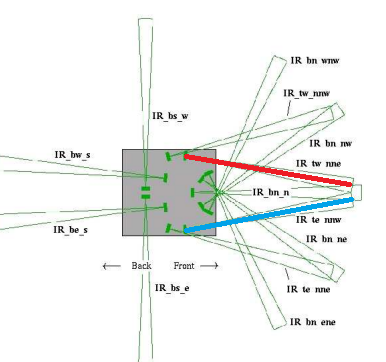
\includegraphics{robot2.png}

\subsection{Sensor-validate}

Mark skriver noget?

\end{document}
